

%----------------------------------------------------------------------------------------
%	Corporate Design 2016 Poster
%----------------------------------------------------------------------------------------
%   Last update 05.09.2017 by Reiner Dietz (mailto: reiner.dietz@simtech.uni-stuttgart.de)
%	Last update 17.11.2016 by Mirco Altenbernd.
%
%	For questions or Bug-Reports
%	mailto: mirco.altenbernd@ians.uni-stuttgart.de
%
%----------------------------------------------------------------------------------------
\documentclass[final,hyperref={pdfpagelabels=false},table]{beamer}
%----------------------------------------------------------------------------------------
\usetheme[a0,simtech]{CDP} % Define DIN-size (available: a0, a1, a2, a3, a4) and other options: german, simtech, compactbib
\usepackage[english]{babel}
\usepackage{ragged2e}
\usepackage{blindtext}
\usepackage{amsmath}

%Mathesymbole
\usepackage{amsmath, amsthm, amssymb}
\usepackage{mathrsfs} 

%Schriftarte
\usepackage{times}

%Einbinden von Grafiken
\usepackage{pdfpages}
\usepackage{graphicx}
\usepackage{epstopdf}
%subfigures
\usepackage{subcaption}

%Schriftarten und Symbole
\usepackage{amsfonts}
\usepackage{amssymb}
%\usepackage{bbold}

%Theoreme, Sätze etc.
\usepackage{amsthm}

%Erlaube Seitenumbrüche in \align-Umgebung
\allowdisplaybreaks

%diagonale Linie für Tabelle
\usepackage{diagbox}

%durchstreichen
\usepackage{ulem}

%für autoref
\usepackage{hyperref}

%up Variante griechischer Buchstaben
\usepackage{upgreek}

%ToDo Kommentare
\usepackage{todonotes}

%Algortihms
\usepackage{algorithm}
\usepackage[noend]{algpseudocode}

% a / b fractions 
\usepackage{nicefrac}

%Tikz
\usepackage{tikz}

\usepackage{color}




\graphicspath{{../gfx/}}

%----------------------------------------------------------------------------------------
%   Helpful things and options
%----------------------------------------------------------------------------------------

% table settings and commands for a suiting table style
\usepackage{xparse}
%\DeclareExpandableDocumentCommand{\BodyCell}{m}{\cellcolor{[1,1,1]} #1}
%\DeclareExpandableDocumentCommand{\HeadCell}{m}{\cellcolor{CD01} \color{white} \textbf{#1}}
\DeclareExpandableDocumentCommand{\BodyCell}{m}{\cellcolor{white} #1}
\DeclareExpandableDocumentCommand{\HeadCell}{m}{\cellcolor{white} \color{black} #1}
\makeatletter
\def\arraystretch{1.1}
\arrayrulecolor{white}
\makeatother

% numbered captions
\setbeamertemplate{caption}[numbered]{}

%colors
\definecolor{mittelblau}{RGB}{32,86,174}

%----------------------------------------------------------------------------------------
%   Title - Parameter
%----------------------------------------------------------------------------------------

% The Poster title
\setTitle{High-Dimensional Battleship-\\[10pt] 
          \huge{discretization methods as \\[10pt]strategies}}

% The Poster subtitle
%\setSubTitle{SimTech}

% Logo subtext (uncomment for Germany-Subtext with english logo)
%\setLogoText{SimTech Cluster of Excellence}
%\setLogoText{Cluster of Excellence in Simulation Technology}



% Institute information/address
\setInst{Institut for Parallel and Distributed Systems (IPVS)\\[2pt]
Simulation Software Engineering\\[2pt]
Universitätsstr. 38, D-70569 Stuttgart, Germany \\[2pt]
schniccr@ipvs.uni-stuttgart.de\\[2pt]
kreittds@ipvs.uni-stuttgart.de
}

% Author name
%\setName{\mbox{Michael Rehme}  \\[4pt] Dirk Pflüger}
\setName{\large{\underline{Christopher}\\[4pt] \underline{Schnick}\\[4pt]  \ \underline{Dennis}\\[4pt] \underline{Kreittner}\\[1pt]  \  Dirk \\[4pt] Pflüger}}

% uncommand for individual footer layout
 \setFooter{
 \begin{tikzpicture}[remember picture,overlay]
     %left aligned footer-content (image)
     \node[anchor=south west, align=left, yshift=0.01\paperwidth, xshift=0.066\paperwidth] at (current page.south west) {
       
\includegraphics[height=0.035\paperheight]{../gfx/ipvs_logo.png}
       \qquad
       
\includegraphics[height=0.035\paperheight]{../gfx/sgslogo-250x250.png}
       %\includegraphics[height=0.035\paperheight]{mathebanner.pdf}
     };
     %center aligned footer-content (image)
     \node[anchor=south, align=center, yshift=0.01\paperwidth, xshift=0] at (current page.south) {
       % 
\includegraphics[height=0.035\paperheight]{logo_simtech.pdf}
     };
     %center aligned footer-content (text) - yshift may be modified for alignment
     \node[anchor=south, align=center, yshift=0.025\paperwidth, xshift=0] at (current page.south) {
       % {\bfseries\large www.sfbtrr75.de}\\
       % {\bfseries\large www.simtech.uni-stuttgart.de}
     };
     %right aligned footer-content (image)
     %\node[anchor=south east, align=right, yshift=0.01\paperwidth, xshift=-0.066\paperwidth] at (current page.south east) {
     %  
\includegraphics[height=0.035\paperheight]{../gfx/logo_simtech.pdf}
     %};
 \end{tikzpicture}
 }

%----------------------------------------------------------------------------------------
%   Content (begin)
%----------------------------------------------------------------------------------------

\begin{document}

\begin{frame}
\centering
\begin{columns}[T]
\begin{column}{\colCWidth}

%----------------------------------------------------------------------------------------
%   Content, left (begin)
%----------------------------------------------------------------------------------------

\justifying
\section{Motivation and Approach}
Objective: \textbf{Investigate} the \textbf{functionality} of high-dimensional battleships. \textbf{Realize} and \textbf{compare} possible shooting \textbf{strategies} based on discretization methods. The general idea for this topic comes from \cite{MF}.
\begin{itemize} 
\item Adapt classic battleship to a \textbf{high-dimensional hypercube}.
\item Redefine terms like \textbf{ship, flee}t and shooting \textbf{strategies}.
\item Evaluation of strategies requires many sample fleets and even more ships.
\item A \textbf{Monte-Carlo approach} reduces the computation cost significantly while still allowing a decent impression of the quality of the strategy.
\item Firstly we use an algorithm to compute the number of shots to sink a random ship.
\end{itemize}

\begin{algorithm}[H]
	\caption*{Calculating number of shots/turns to sink a random ship}\label{alg:calcTurns}
	\begin{algorithmic}
		\Procedure{calcTurns}{$n,\text{strat}$}
		\State $\Omega_L = generate\_random\_ships(n)$  
		\Comment{Generate $n$ random ships}
		\State $turns = [1,\dots,|C_{all}|]$
		\State $sum = 0$
		\For{$i=1,\dots,n$} 
		\State $min = min_{c\in cells(\Omega_L[i])}I_{strat}(c)$
		\State $turns[min]++$
		\EndFor
		\State \textbf{return} $turns$
		\EndProcedure
	\end{algorithmic}
\end{algorithm}

\begin{itemize}
\item By using the previous algorithm we can calculate the \textbf{distribution function} of the strategy for a sample.
\item The Monte-Carlo approach now assumes that this distribution resembles the distribution for all possible ships.
\end{itemize}

\begin{algorithm}[H]
	\caption*{Calculating distribution function of a strategy}\label{alg:evaluateStrat}
	\begin{algorithmic}
		\Procedure{evaluate\_strategy}{$n, \text{strat}$}
		\State $turns = calculate\_turns(n, \text{strat})$;
		\State $ship\_sum=0$;
		\For{$i=1,\dots,|C_{all}|$}
		\State $ships=turns[i]$;
		\State $ship\_sum += ships$;
		\State $P(\mathbf{T}^{\Omega_L}_{\text{strat}} \leq i)=\frac{ship\_sum}{n}$;
		\State $P(\mathbf{X}^{F_{all}}_{\text{strat}} \leq i)=\frac{2^{\left(P(\mathbf{T}^{\Omega_L}_{\text{strat}} \leq i) * |L_{all}|\right)} - 1}{2^{|L_{all}|} - 1}$;
		\EndFor
		\EndProcedure
	\end{algorithmic}
\end{algorithm}


\section{Strategies}
For shooting strategies we want to orientate us at \textbf{discretization methods} since they are easily adapted to high dimensions. For that matter we came up with \textbf{five different strategies}. In general grid startegies use the following partitioning:
\begin{figure}[h]
	\centering
	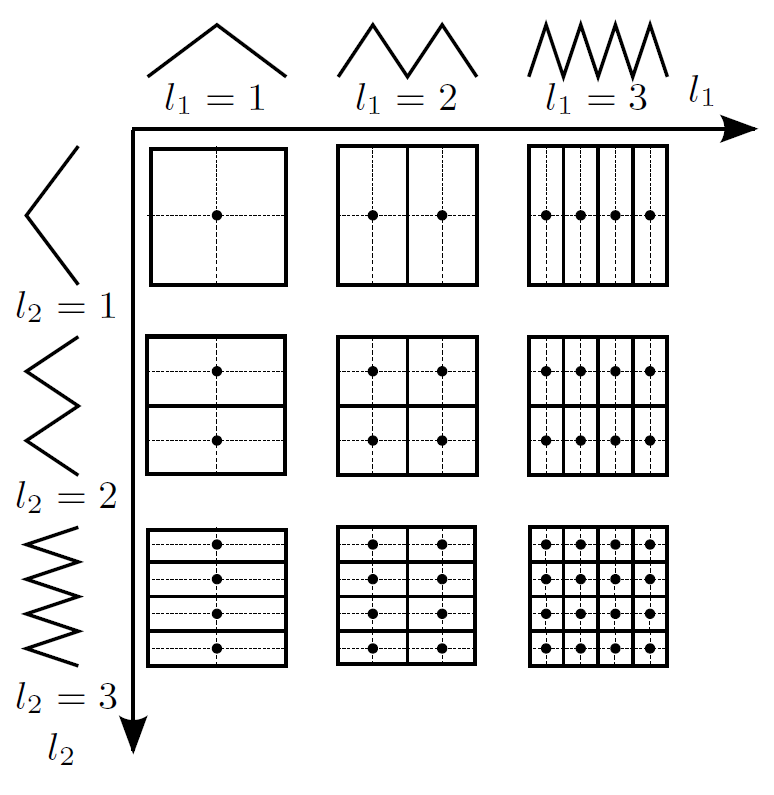
\includegraphics[width=0.3\textwidth]{../gfx/Grids03.png}
	\caption{Halving of the grid coordinates}
\end{figure}
\begin{itemize}
\item Random Strategy: Shoots at a random cell of the hypercube. This is the closest strategy to the reality since most battleship players target random cells.
\item Full Grid Strategy: Shoots cells according to the discretization given by a full grid.
\end{itemize}



%implemented the following algorithm to create a variance adaptive level structure:
%\begin{itemize}
%\item On each level $\ell$ calculate the variance $v_\ell$.
%\item Calculate $\Delta_m$, the surplus of level $m$, by combining the variances in $\Psi_m$, the set of all predecessors of level $m$.
%\item For all potential new levels $n$ calculate their priority $p_n$ from their direct predecessors $\psi_n \subseteq \Psi_n$.
%\item Add the level with highest priority until the maximum number of points is reached.
%\end{itemize}




%\begin{itemize}  	
%\item This refinement algorithm can easily be adapted to other objective values than the variance.
%\end{itemize}

\begin{figure}[h]
\centering
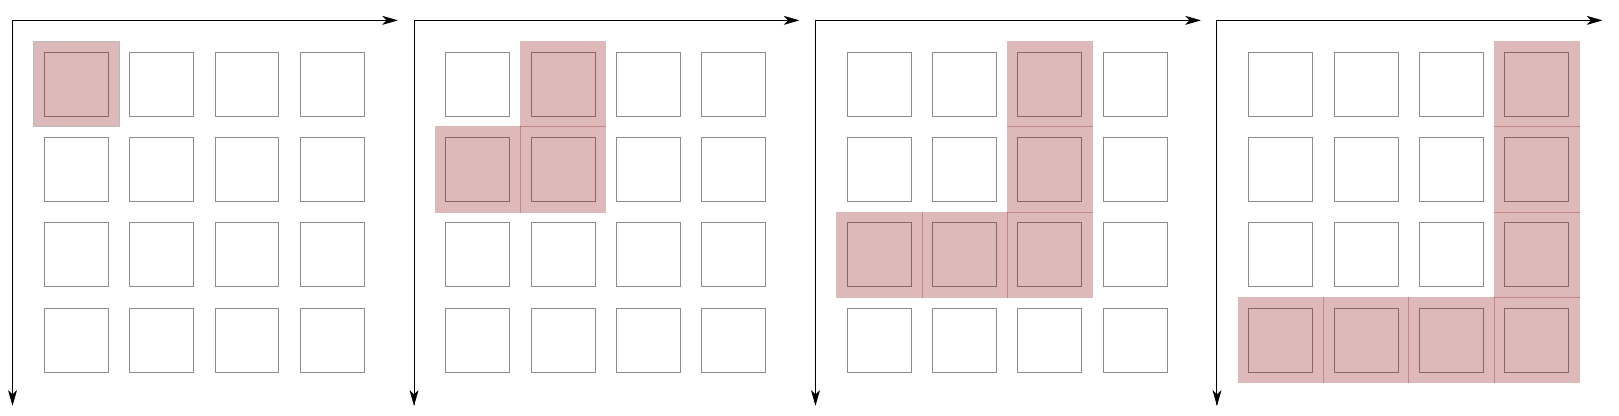
\includegraphics[width=\textwidth]{../gfx/Grids04.png}
\caption{Structure of Full Grid Strategy}
\end{figure}



%----------------------------------------------------------------------------------------
%   Content, left (end)
%----------------------------------------------------------------------------------------

\end{column}
\begin{column}{\colCWidth}

%----------------------------------------------------------------------------------------
%   Content, right (begin)
%----------------------------------------------------------------------------------------

\justifying
\begin{itemize}
	\item Sparse Grid Strategy: Shoots cells according to the discretization given by a sparse grid.
\end{itemize}
\begin{figure}[h]
	\centering
	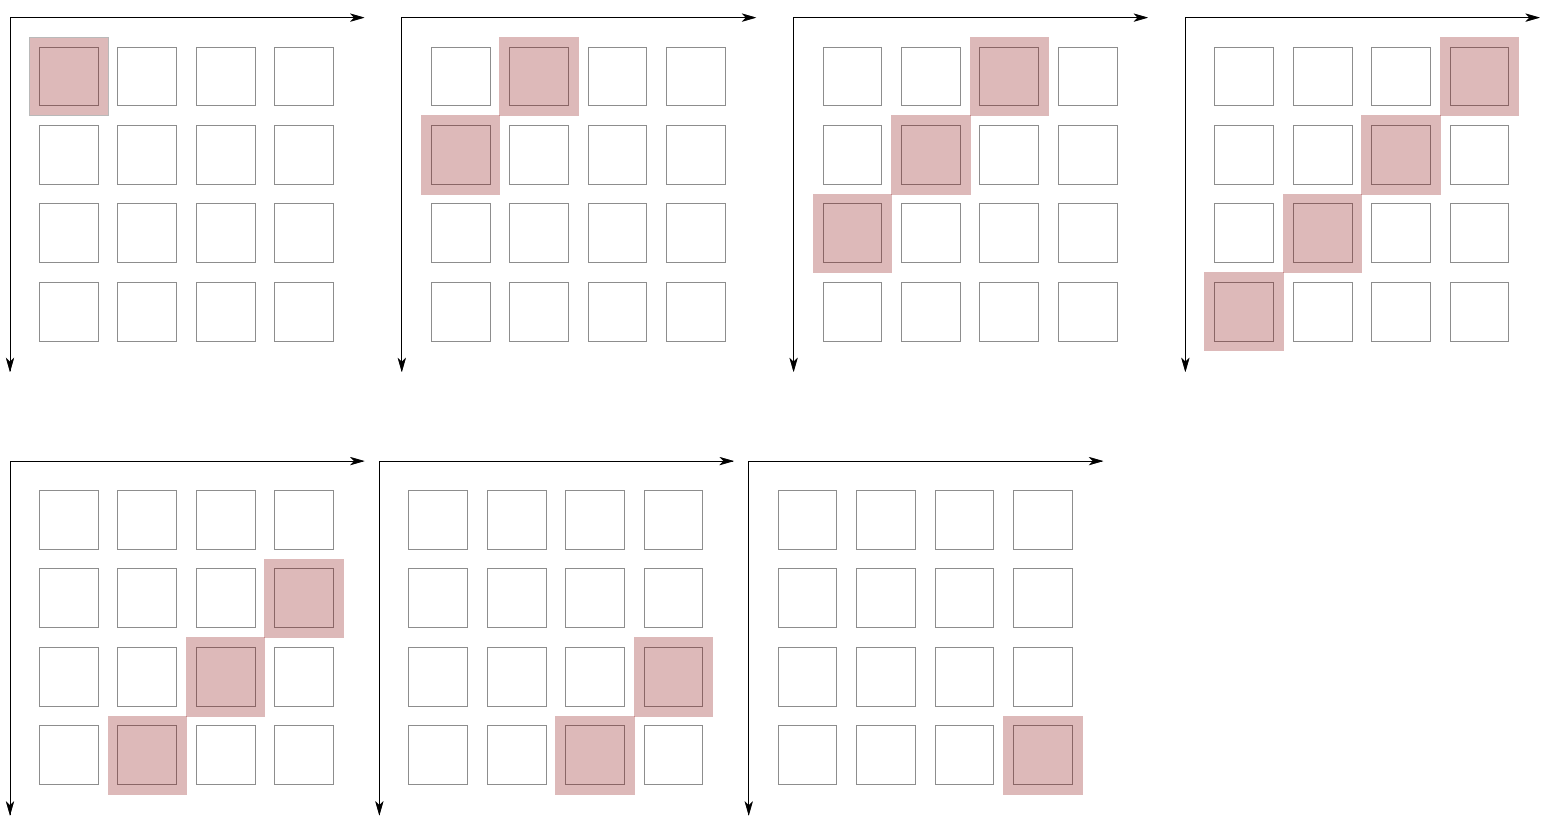
\includegraphics[width=\textwidth]{../gfx/Grids05.png}
	\caption{Structure of Sparse Grid Strategy}
\end{figure}
\begin{itemize}
	\item Sobol Strategy: This strategy shoots according to the pseudorandom Sobol number sequence which is based on polynomials in $\mathbb{Z}_2$. The definitions and algorithms are based on \cite{JK}.
	\item Halton Strategy: Here the strategy is based on onedimensional number sequences of fractions of primes which we combine to multidimensional coodinates.
\end{itemize}

\subsection{Results}

After computing the results for the different strategies with varying dimensions and sample sizes we can compare them now. 

\begin{figure}[h]
	\centering
	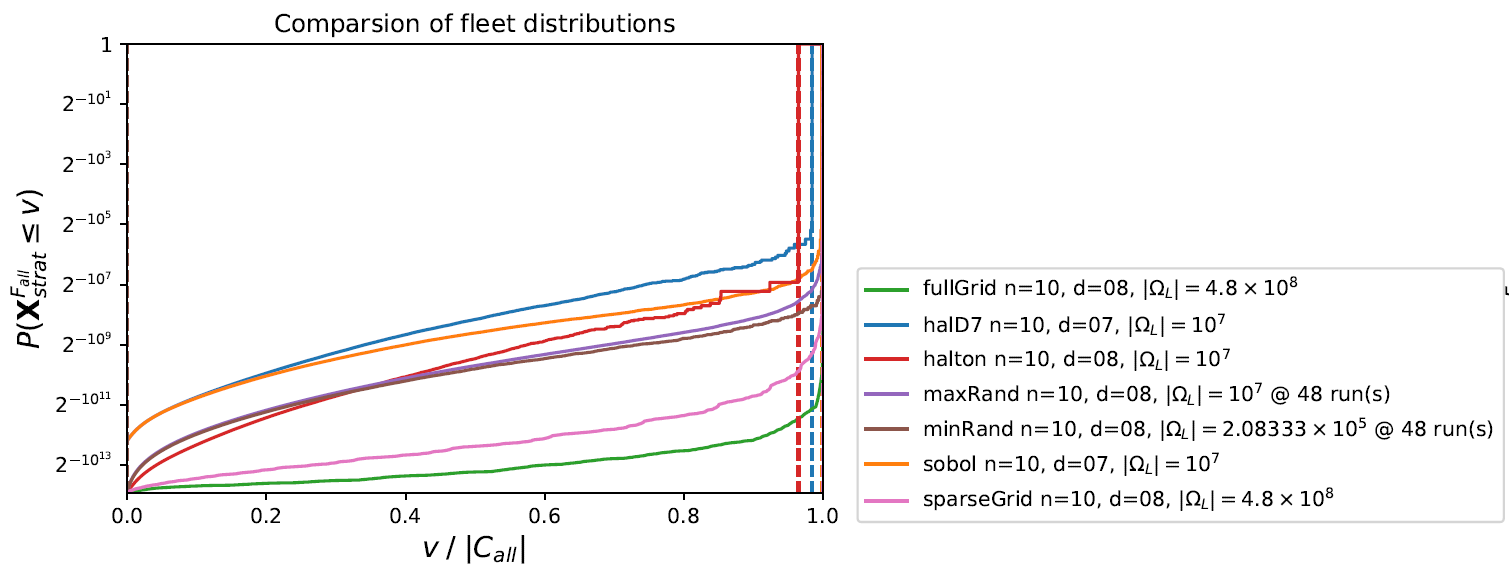
\includegraphics[width=\textwidth]{../gfx/Compare01.png}
	\caption{Comparsion Strategies for random fleet}
	\label{fig:comp01}
\end{figure}

In figure \ref{fig:comp01} we see, that the Halton Strategy for 7 dimensions overtakes Sobol. This implies the same for 8 dimensions. Which is why we conclude that the Halton Strategy performs the best out of all the tested strategies. Note: The goal of the curves is to reach the top as fast as possible.
This conclusion is also confirmed by figure \ref{fig:comp02} in which the total number of necessary shots is lowest for the Halton Strategy.

\begin{figure}[h]
	\centering
	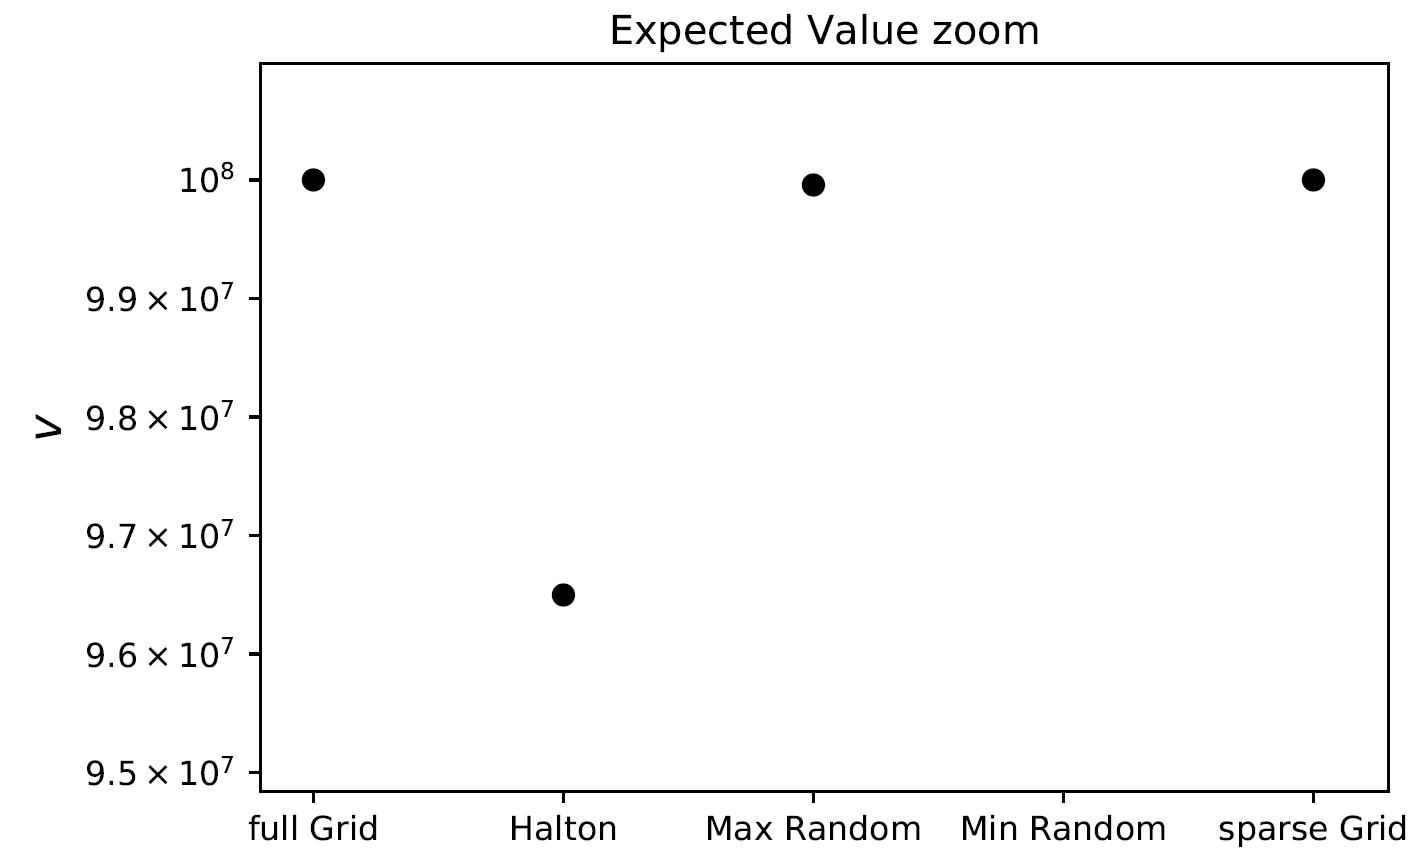
\includegraphics[width=0.7\textwidth]{../gfx/Compare02.png}
	\caption{Comparsion number of shots for random fleet}
	\label{fig:comp02}
\end{figure}



%\nocite{*} %shows all content within the bibliography file
\section{References}
\normalem %suppresses underlines in bibliography
\bibliography{../literature/references.bib}


%----------------------------------------------------------------------------------------
%   Content, right (end)
%----------------------------------------------------------------------------------------

\end{column}
\end{columns}

\end{frame}
\end{document}

%----------------------------------------------------------------------------------------
%   Content (end)
%----------------------------------------------------------------------------------------
